\documentclass[11pt]{article}

% ----------------------------------------------------------------------
%  CHE374  Economic Analysis and Decision Making
%  Lecture notes, Weeks 1 to 4
% ----------------------------------------------------------------------

\usepackage[margin=1in]{geometry}
\usepackage{amsmath,amssymb,amsthm}
\usepackage{xcolor}
\usepackage{graphicx}
\usepackage{booktabs}
\usepackage[most]{tcolorbox}
\usepackage{titlesec}
\usepackage[font={small},labelformat=empty]{caption}
\usepackage{enumitem}
\usepackage{mathtools}
\usepackage{tikz}
\usepackage{pgfplots}
\pgfplotsset{compat=1.17}
\usetikzlibrary{arrows.meta,positioning,decorations.pathreplacing,calc,shapes.misc}

% ---- colour palette ----------------------------------------------------
\definecolor{cHead}{HTML}{14365C}    % navy  (headings)
\definecolor{cTerm}{HTML}{0F7173}    % teal  (key concept words)
\definecolor{cBox}{HTML}{0F7173}     % teal  (formula box frame)
\definecolor{cBoxbg}{HTML}{EAF5F5}   % light teal (formula box fill)
\definecolor{cNote}{HTML}{B07A1E}    % amber (side notes)
\definecolor{cNotebg}{HTML}{FBF4E4}  % light amber
\definecolor{posflow}{RGB}{210,125,20}  % receipts (up arrows)
\definecolor{negflow}{RGB}{40,90,170}   % disbursements (down arrows)
\definecolor{accent}{RGB}{150,30,30}

% ---- headings ----------------------------------------------------------
\titleformat{\section}{\normalfont\Large\bfseries\color{cHead}}{\color{cHead}\thesection}{0.6em}{}
\titleformat{\subsection}{\normalfont\large\bfseries\color{cHead}}{}{0em}{}
\titleformat{\subsubsection}{\normalfont\normalsize\bfseries\color{cHead}}{}{0em}{}
\captionsetup{font={small,color=black!60}}

% ---- key-term command --------------------------------------------------
\newcommand{\term}[1]{\textbf{\textcolor{cTerm}{#1}}}

% ---- general-formula box + variable legend -----------------------------
\newtcolorbox{genform}{enhanced,colback=cBoxbg,colframe=cBox,
  boxrule=0.6pt,arc=3pt,left=8pt,right=8pt,top=5pt,bottom=6pt,
  title=General formula,fonttitle=\bfseries\small,coltitle=white}
\newcommand{\where}[1]{\par\smallskip{\footnotesize\color{black!72}\textit{where }#1}}

% ---- side note box -----------------------------------------------------
\newtcolorbox{noteboxenv}{enhanced,breakable,colback=cNotebg,colframe=cNote,
  boxrule=0.5pt,arc=3pt,left=8pt,right=8pt,top=4pt,bottom=4pt}
\newcommand{\fillnote}[1]{\begin{noteboxenv}\small\textcolor{cNote}{$\blacktriangleright$}\ #1\end{noteboxenv}}

% ---- cash flow timeline helpers ---------------------------------------
\newcommand{\cfaxis}[1]{\draw[-{Latex[length=2mm]},thick] (-0.3,0) -- (#1,0);}
\newcommand{\up}[3]{\draw[-{Latex[length=2mm]},very thick,posflow] (#1,0) -- (#1,#2) node[above]{\small #3};}
\newcommand{\dn}[3]{\draw[-{Latex[length=2mm]},very thick,negflow] (#1,0) -- (#1,-#2) node[below]{\small #3};}
\newcommand{\tick}[2]{\fill (#1,0) circle (1.3pt); \node[below=2pt] at (#1,0) {\small #2};}

\setlength{\parindent}{0pt}
\setlength{\parskip}{4pt}

\begin{document}

% ---- title -------------------------------------------------------------
\begin{center}
  {\LARGE\bfseries\color{cHead} CHE374: Economic Analysis and Decision Making}\\[4pt]
  {\large\color{cTerm} Lecture Notes \;$\cdot$\; Weeks 1 to 5}\\[6pt]
  {\normalsize Rhyl \;$\cdot$\; Fall 2026}
\end{center}
\vspace{2pt}
{\color{cHead}\hrule height 1pt}
\vspace{6pt}

\tableofcontents
\vspace{6pt}
{\color{cHead!40}\hrule}
\bigskip

% ======================================================================
\section{Lecture One: Time Value of Money}
% ======================================================================

Concept of time value of money: borrowing money has a cost for the borrower,
and lending money should create value for the lender. You get back the
original money plus interest, and the \term{interest rate} is
\[
i = \frac{\text{interest}}{\text{principal}}.
\]

Notation:
\begin{itemize}[nosep]
  \item $P$: present value
  \item $F$: future amount
  \item $i$: interest rate
\end{itemize}

So over one period:
\[
F = P + Pi, \qquad\Longrightarrow\qquad F = P(1+i).
\]

\begin{figure}[h]
\centering
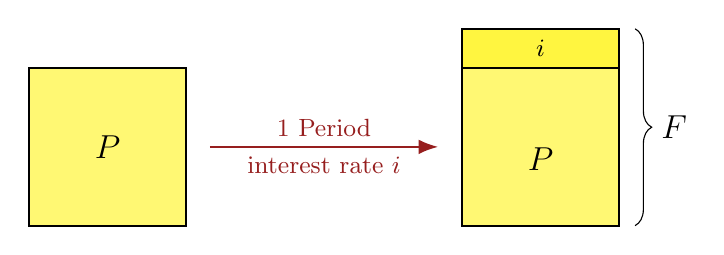
\begin{tikzpicture}[scale=1]
  \draw[thick,fill=yellow!55] (0,0) rectangle (2,2);
  \node at (1,1) {\large $P$};
  \draw[-{Latex[length=2.5mm]},thick,accent] (2.3,1) -- (5.2,1)
        node[midway,above]{\small 1 Period}
        node[midway,below]{\small interest rate $i$};
  \draw[thick,fill=yellow!55] (5.5,0) rectangle (7.5,2);
  \node at (6.5,0.85) {\large $P$};
  \draw[thick,fill=yellow!75] (5.5,2) rectangle (7.5,2.5);
  \node at (6.5,2.25) {\small $i$};
  \draw[decorate,decoration={brace,amplitude=6pt}] (7.7,2.5) -- (7.7,0)
        node[midway,right=6pt]{\large $F$};
\end{tikzpicture}
\caption*{One period growth: the principal $P$ earns interest $Pi$, giving $F=P(1+i)$.}
\end{figure}

\subsection*{Interest rates (in \%)}
The rate depends on the type of investment:
\begin{enumerate}[nosep]
  \item \term{T-Bill} (short term loan to the Bank of Canada): typically earns
        the lowest return but is considered risk free.
  \item \term{Bonds} (lending money to a provincial or Canadian government):
        pay a slightly higher interest rate.
  \item \term{Personal loans or loans to small businesses:} riskier, but a
        significantly higher interest rate.
\end{enumerate}

Factors that affect the rate:
\begin{enumerate}[nosep]
  \item Inflation
  \item Credit (default) risk
  \item Liquidity risk
  \item Maturity
\end{enumerate}

\subsection*{Simple vs.\ compound interest}
Notation again:
\begin{itemize}[nosep]
  \item $P$: present (principal)
  \item $F_N$: future amount in year $N$
  \item $i$: interest rate
  \item $I$: interest amount
\end{itemize}

\term{Simple interest} applies only to the original principal:
\[
F_N = P(1 + Ni).
\]

\term{Compound interest} applies to the principal and all interest accrued so
far (e.g.\ mortgages, credit card debt):
\[
F_N = P(1+i)^{N}.
\]

For the same rate $r$ per year, the more frequently you compound (the bigger
$m$) the more you earn.

\begin{figure}[h]
\centering
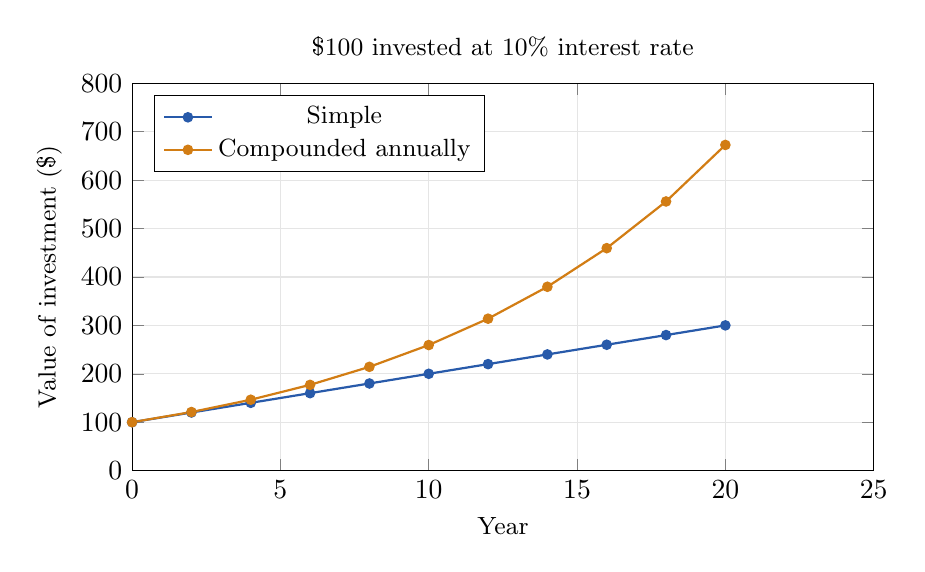
\begin{tikzpicture}
\begin{axis}[
  width=11cm, height=6.5cm,
  title={\small \$100 invested at 10\% interest rate},
  xlabel={\small Year}, ylabel={\small Value of investment (\$)},
  xmin=0, xmax=25, ymin=0, ymax=800,
  xtick={0,5,10,15,20,25}, ytick={0,100,...,800},
  legend pos=north west, legend style={font=\small},
  grid=both, grid style={gray!20},
]
\addplot[negflow,thick,mark=*,mark size=1.5pt,domain=0:20,samples=11] {100*(1+0.1*x)};
\addlegendentry{Simple}
\addplot[posflow,thick,mark=*,mark size=1.5pt,domain=0:20,samples=11] {100*(1.1)^x};
\addlegendentry{Compounded annually}
\end{axis}
\end{tikzpicture}
\caption*{Simple interest grows linearly; compound interest grows exponentially.}
\end{figure}

\subsection*{Effective interest rate}
The \term{effective interest rate} is the equivalent interest rate of an account
that is compounded just once over a year:
\[
i_e = \left(1 + \frac{r}{m}\right)^{m} - 1.
\]
Here we compound multiple times per year:
\begin{itemize}[nosep]
  \item $r$: nominal interest rate (for one year),
  \item allowed to compound $m$ times (subperiods) per year,
  \item $F = P\left(1+\dfrac{r}{m}\right)^{m}$,
  \item $\dfrac{r}{m} = i_s =$ subperiod rate.
\end{itemize}

\subsection*{Continuous compounding}
\[
i_e = \lim_{m\to\infty}\left(1+\frac{r}{m}\right)^{m} - 1 = e^{\,r} - 1.
\]

% ======================================================================
\section{Week Two: Cash Flows and Equivalence}
% ======================================================================

\subsection*{Categories of cash flow}

\textbf{1. At the start:}
\begin{itemize}[nosep]
  \item \term{First cost} (capital cost).
\end{itemize}

\textbf{2. During a project (investment):}
\begin{itemize}[nosep]
  \item \term{Revenue:} we will have some revenues or savings (car example).
  \item \term{O\&M} (operation and maintenance): e.g.\ car insurance or fuel.
  \item \term{Overhaul}, a major expenditure: e.g.\ an engine requires an
        overhaul about half way through its life.
\end{itemize}

\textbf{3. At the end:}
\begin{itemize}[nosep]
  \item \term{Salvage value:} net receipt at the end, e.g.\ from the sale of a
        piece of equipment (sell the car).
  \item \term{Scrap value:} value in the materials the item is made of.
  \item \term{Disposal cost:} the cost to dispose of a waste when it is no
        longer usable.
\end{itemize}

\subsection*{Cash flow diagrams}
Time $0$ is the beginning of period one. A cash flow occurring during a period is
accrued at the \emph{end} of that period.

\begin{figure}[h]
\centering
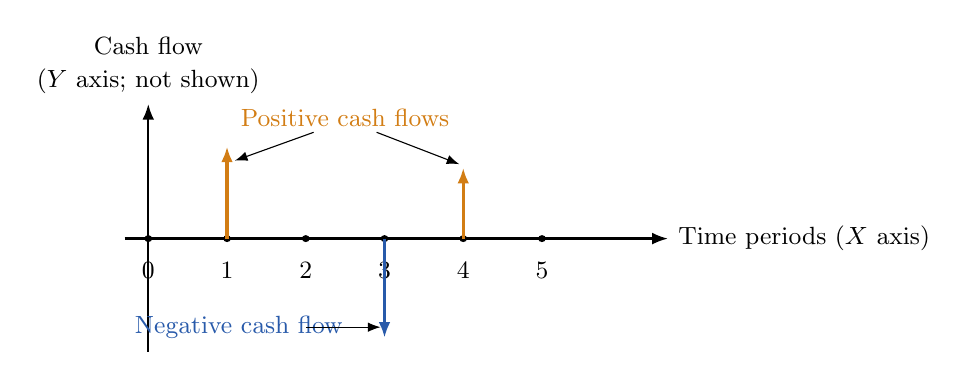
\begin{tikzpicture}[yscale=0.9]
  \draw[-{Latex[length=2mm]},thick] (-0.3,0) -- (6.6,0) node[right]{\small Time periods ($X$ axis)};
  \draw[-{Latex[length=2mm]},thick] (0,-1.6) -- (0,1.9) node[above,align=center]{\small Cash flow\\\small ($Y$ axis; not shown)};
  \foreach \x/\n in {0/0,1/1,2/2,3/3,4/4,5/5} {\fill (\x,0) circle (1.4pt); \node[below=5pt] at (\x,0){\small \n};}
  \draw[-{Latex[length=2mm]},very thick,posflow] (1,0) -- (1,1.3);
  \draw[-{Latex[length=2mm]},very thick,posflow] (4,0) -- (4,1.0);
  \node[align=center,posflow] at (2.5,1.7) {\small Positive cash flows};
  \draw[-{Latex[length=1.6mm]},thin] (2.1,1.5) -- (1.1,1.1);
  \draw[-{Latex[length=1.6mm]},thin] (2.9,1.5) -- (3.95,1.05);
  \draw[-{Latex[length=2mm]},very thick,negflow] (3,0) -- (3,-1.4);
  \node[align=center,negflow] at (1.15,-1.25) {\small Negative cash flow};
  \draw[-{Latex[length=1.6mm]},thin] (2.0,-1.25) -- (2.95,-1.25);
\end{tikzpicture}
\caption*{Up arrows are receipts (positive); the down arrow is a disbursement (negative).}
\end{figure}

\subsection*{Standard cash flow patterns}

\textbf{1. Single payment.}
\begin{figure}[h]
\centering
\begin{tikzpicture}[yscale=0.9]
  \cfaxis{8}
  \foreach \x/\n in {0/0,1/1,2/2,4/$N-1$,5.5/$N$,7/$N+1$} {\tick{\x}{\n}}
  \node at (3,0) {$\sim$};
  \up{5.5}{1.6}{$F$}
\end{tikzpicture}
\caption*{A single future amount $F$ received at time $N$.}
\end{figure}

\textbf{2. Perpetuity:} an annuity that pays $A$ forever.
\[
P = \frac{A}{i}.
\]
\begin{figure}[h]
\centering
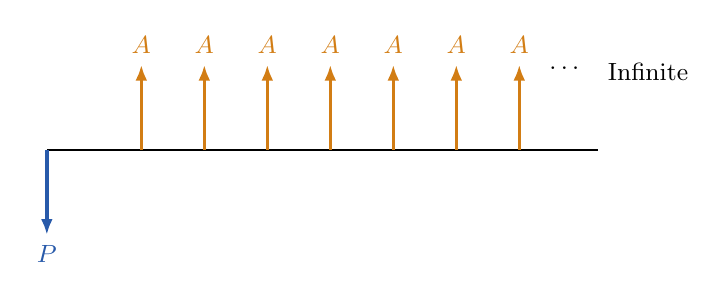
\begin{tikzpicture}[yscale=0.9]
  \draw[thick] (0,0) -- (7,0);
  \foreach \x in {1.2,2,2.8,3.6,4.4,5.2,6} {\up{\x}{1.2}{$A$}}
  \node at (6.6,1.15) {\small \dots};
  \node[right] at (7,1.1) {\small Infinite};
  \dn{0}{1.2}{$P$}
\end{tikzpicture}
\caption*{Perpetuity: a level payment $A$ that never ends, $P=A/i$.}
\end{figure}

\textbf{3. Annuity:} a perpetuity but only for $N$ periods.
\begin{figure}[h]
\centering
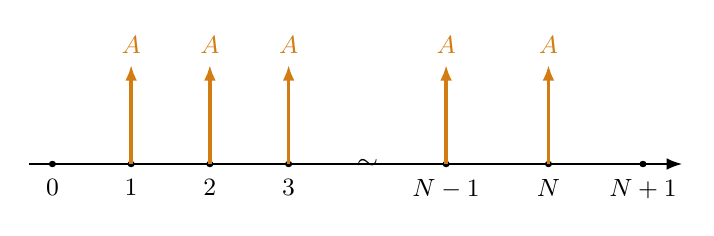
\begin{tikzpicture}[yscale=0.9]
  \cfaxis{8}
  \foreach \x/\n in {0/0,1/1,2/2,3/3,5/$N-1$,6.3/$N$,7.5/$N+1$} {\tick{\x}{\n}}
  \node at (4,0) {$\sim$};
  \foreach \x in {1,2,3,5,6.3} {\up{\x}{1.4}{$A$}}
\end{tikzpicture}
\caption*{Annuity: a level payment $A$ for $N$ periods.}
\end{figure}

\textbf{4. Arithmetic gradient.} We assume the first cash flow happens at period
two, so $i$ starts at period one; we treat the constant first part as an annuity
$A'$ and add the growing part $G$.
\begin{figure}[h]
\centering
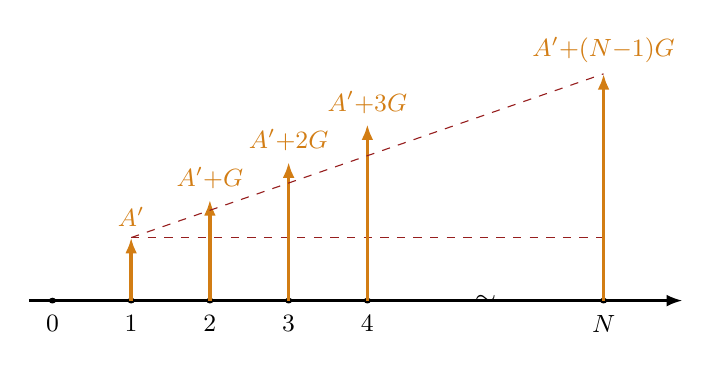
\begin{tikzpicture}[yscale=0.8]
  \draw[-{Latex[length=2mm]},thick] (-0.3,0) -- (8,0);
  \foreach \x/\n in {0/0,1/1,2/2,3/3,4/4,7/$N$} {\tick{\x}{\n}}
  \node at (5.5,0) {$\sim$};
  \draw[dashed,accent] (1,1) -- (7,1);
  \up{1}{1}{$A'$}
  \up{2}{1.6}{$A'{+}G$}
  \up{3}{2.2}{$A'{+}2G$}
  \up{4}{2.8}{$A'{+}3G$}
  \up{7}{3.6}{$A'{+}(N{-}1)G$}
  \draw[dashed,accent] (1,1) -- (7,3.6);
\end{tikzpicture}
\caption*{Arithmetic gradient: a base annuity $A'$ plus a linear growth $G$ each period.}
\end{figure}

\textbf{5. Geometric gradient:} each cash flow grows by a constant factor
$(1+g)$.
\begin{figure}[h]
\centering
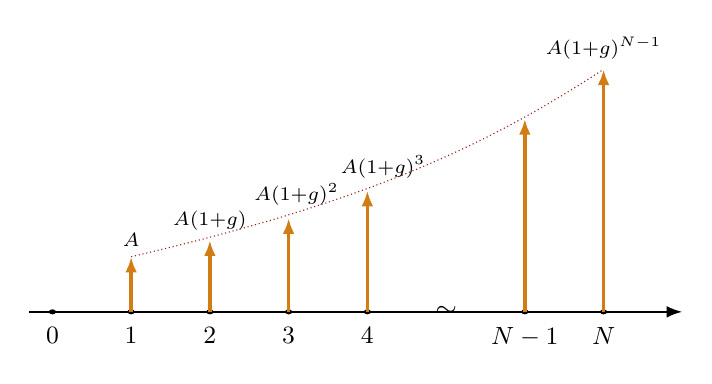
\begin{tikzpicture}[yscale=0.7]
  \draw[-{Latex[length=2mm]},thick] (-0.3,0) -- (8,0);
  \foreach \x/\n in {0/0,1/1,2/2,3/3,4/4,6/$N-1$,7/$N$} {\tick{\x}{\n}}
  \node at (5,0) {$\sim$};
  \up{1}{1}{} \up{2}{1.3}{} \up{3}{1.7}{} \up{4}{2.2}{} \up{6}{3.5}{} \up{7}{4.4}{}
  \node[above] at (1,1) {\scriptsize $A$};
  \node[above] at (2,1.3) {\scriptsize $A(1{+}g)$};
  \node[above] at (3.1,1.75) {\scriptsize $A(1{+}g)^2$};
  \node[above] at (4.2,2.25) {\scriptsize $A(1{+}g)^3$};
  \node[above] at (7,4.4) {\scriptsize $A(1{+}g)^{N-1}$};
  \draw[densely dotted,accent] (1,1) .. controls (4,2) and (5.5,3) .. (7,4.4);
\end{tikzpicture}
\caption*{Geometric gradient: each payment is $(1+g)$ times the one before.}
\end{figure}

\subsection*{Three kinds of equivalence}

\textbf{1. \term{Mathematical equivalence}:} two cash flows $P_t$ at time $t$ and
$F_{t+N}$ (or $F_{t+N+M}$) are equivalent with respect to the interest rate:
\[
P_t = \frac{F_{t+N}}{(1+i)^{N}}.
\]
\begin{figure}[h]
\centering
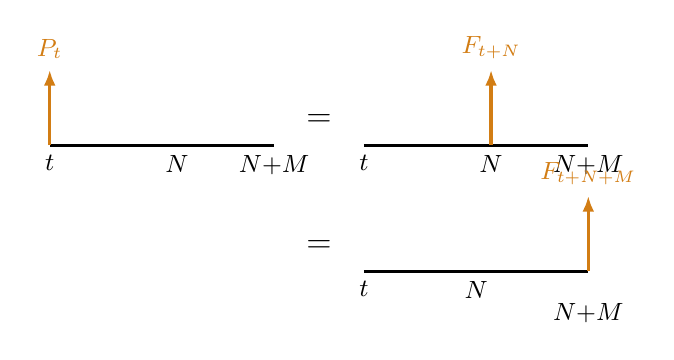
\begin{tikzpicture}[yscale=0.8,xscale=0.95]
  \draw[thick] (0,0) -- (3,0);
  \up{0}{1.2}{$P_t$}
  \node[below] at (0,0){\small $t$}; \node[below] at (1.7,0){\small $N$}; \node[below] at (3,0){\small $N{+}M$};
  \node at (3.6,0.4) {\large $=$};
  \draw[thick] (4.2,0) -- (7.2,0);
  \up{5.9}{1.2}{$F_{t+N}$}
  \node[below] at (4.2,0){\small $t$}; \node[below] at (5.9,0){\small $N$}; \node[below] at (7.2,0){\small $N{+}M$};
  \node at (3.6,-1.6) {\large $=$};
  \draw[thick] (4.2,-2) -- (7.2,-2);
  \draw[-{Latex[length=2mm]},very thick,posflow] (7.2,-2) -- (7.2,-0.8) node[above]{\small $F_{t+N+M}$};
  \node[below] at (4.2,-2){\small $t$}; \node[below] at (5.7,-2){\small $N$}; \node[below] at (7.2,-2.35){\small $N{+}M$};
\end{tikzpicture}
\caption*{The same value, seen at time $t$, at $N$, and at $N+M$.}
\end{figure}

\textbf{2. \term{Market equivalence}:} the idea that one can exchange cash flows
between present and future amounts.

\textit{Example.} A Treasury Bill (T-bill) is a short term government debt
obligation backed by the government, with a maturity of one year or less.
T-bills are usually sold in denominations of \$1{,}000. If a \$1000 T-bill due to
mature in 6 months is currently selling for \$990.10, that means some investors
holding the T-bill are willing to sell at this price while others are willing to
buy at this price. The ``market'' has agreed that the appropriate interest rate
is 1\% over 6 months:
\[
990.15\,(1 + 0.01) \approx 1000.
\]
\begin{figure}[h]
\centering
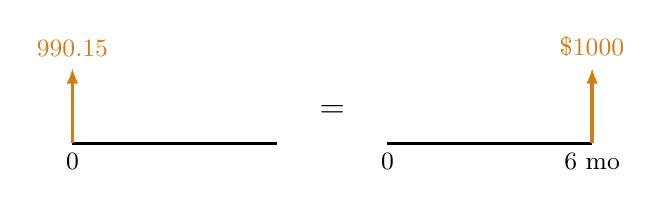
\begin{tikzpicture}[yscale=0.8]
  \draw[thick] (0,0) -- (2.6,0);
  \up{0}{1.2}{$990.15$}
  \node[below] at (0,0){\small 0};
  \node at (3.3,0.5){\large $=$};
  \draw[thick] (4,0) -- (6.6,0);
  \up{6.6}{1.2}{\$1000}
  \node[below] at (4,0){\small 0}; \node[below] at (6.6,0){\small 6 mo};
\end{tikzpicture}
\caption*{\$990.15 today is equivalent to \$1000 in six months at 1\%.}
\end{figure}

\textbf{3. \term{Decisional equivalence}:} indifference of the decision maker
among the available choices.

\subsection*{Factor notation}
$(X/Y, i\%, N)$, where $X$ and $Y$ are chosen from the cash flow symbols
$P, F, A, G$. If you have $Y$ multiplied by a factor, you get the equivalent
value of $X$, e.g.\ $P = F(P/F, i, N)$.

\begin{align*}
(A/P, i, N) &= \frac{1}{(P/A, i, N)}\\[2pt]
(F/P, i, N) &= (1+i)^{N}\\[2pt]
(P/F, i, N) &= (1+i)^{-N}\\[2pt]
P = A\,(P/A, i, N) &= A\!\left(\frac{1}{i} - \frac{1}{i(1+i)^{N}}\right)\\[2pt]
(P/G, i, N) &= \frac{1}{i^{2}}\left(1 - \frac{1+iN}{(1+i)^{N}}\right)
             = \frac{(1+i)^{N} - 1 - iN}{i^{2}(1+i)^{N}}\\[2pt]
(P/\mathrm{Geom}, i, g, N) &= \frac{1 - \left(\frac{1+g}{1+i}\right)^{N}}{i - g}
\end{align*}

\fillnote{Small corrections to the written factors: continuous compounding gives
$e^{r}-1$ (not $s^{r}-1$); and the $(P/G)$ factor carries $1/i^{2}$ out front,
not $i/i^{2}$. Everything else matches the standard factor table.}

Or, equivalently, for the geometric gradient:
\[
(P/\mathrm{Geom}, i, g, N) = \frac{(P/A, i^{0}, N)}{1+g},
\qquad\text{where } i^{0} = \frac{1+i}{1+g} - 1.
\]

\textbf{Putting the factors to work:}
\begin{itemize}[nosep]
  \item Annuity: $P = A\,(P/A, i, N)$.
  \item Arithmetic: $P = A\,(P/A, i, N) + G\,(P/G, i, N)$. Do the bottom bracket
        first: the first term is the initial annuity value $A$ that is constant
        starting at $t=1$; the second term is the growing value $G$.
  \item Geometric: $P = \dfrac{A}{1+g}\,(P/A, i^{0}, N)$.
\end{itemize}

% ======================================================================
\section{Week Three: Mortgages and Bonds}
% ======================================================================

\subsection*{Mortgage loan terminology}
Buy a house for \$500k $=$ total value.
\begin{itemize}[nosep]
  \item \term{Principal:} you can borrow up to a certain fraction (e.g.\ \$400k).
  \item \term{Down payment:} the rest of it.
  \item \term{LTV:} loan to value ratio $=\dfrac{P}{\text{total}}$.
  \item \term{Mortgage rate.}
  \item \term{Amortization period:} the agreed time horizon for repayment.
  \item \term{Term:} the agreed interest rate period (the interest rate can
        change between terms).
\end{itemize}

\subsection*{Mortgage Example}
\textit{These examples did not list the formulas, so they are worked out here,
and a general form is given below each part.}

\$500{,}000 home, with a 20\% down payment; mortgage rate is 5\%, 5 year term,
25 year amortization period.

\textbf{(a) What is your monthly payment during this term?}

The principal is $P = 500{,}000 \times 80\% = \$400{,}000$. Since payments are
monthly, use a monthly rate and a monthly count:
\[
i = \frac{5\%}{12}, \qquad N = 25 \times 12 = 300.
\]
\[
A = 400{,}000\,(A/P,\ \tfrac{5\%}{12},\ 300)
  = 400{,}000 \times \frac{i(1+i)^{300}}{(1+i)^{300}-1}
  \approx \boxed{\$2{,}338 \text{ per month}.}
\]

\begin{genform}
\[
A = P\,(A/P,\ i,\ N),\qquad i = \frac{r_{\text{mort}}}{m},\qquad N = Y_{\text{am}}\times m.
\]
\where{$A=$ payment per period;\;
$P=$ principal $=$ (home value)$\times(1-\text{down payment fraction})$;\;
$i=$ periodic rate;\;
$r_{\text{mort}}=$ mortgage rate (annual, nominal);\;
$m=$ payments per year ($m=12$ for monthly);\;
$Y_{\text{am}}=$ amortization period in years;\;
$N=$ total number of payments.}
\end{genform}

\textbf{(b) After the end of the term, the new mortgage rate is 6\%. What is your
new monthly payment?}

Two steps. First find the amount still owed after 5 years (that is, after
$5\times 12 = 60$ payments). Take the original principal forward to year 5 and
subtract the future value of the payments already made:
\[
\text{Amount owed} = 400{,}000\,(F/P,\ \tfrac{5\%}{12},\ 60)
   - 2338\,(F/A,\ \tfrac{5\%}{12},\ 60) \approx \$354{,}320.
\]
This is the principal still outstanding at year 5. Now spread that balance over
the remaining $20 \times 12 = 240$ months at the new rate of $6\%/12$:
\[
A_{\text{new}} = 354{,}320\,(A/P,\ \tfrac{6\%}{12},\ 240)
   \approx \boxed{\$2{,}538 \text{ per month}.}
\]

\begin{genform}
\[
B_{k} = P\,(F/P,\ i,\ k) - A\,(F/A,\ i,\ k),
\qquad
A_{\text{new}} = B_{k}\,(A/P,\ i_{\text{new}},\ N-k).
\]
\where{$B_k=$ balance still owed after $k$ payments;\;
$k = Y_{\text{term}}\times m$ (payments made during the first term);\;
$A=$ the original payment from part (a);\;
$i=r_{\text{mort}}/m$ (old periodic rate);\;
$i_{\text{new}}=r_{\text{new}}/m$ (new periodic rate after the term);\;
$N-k=$ remaining payments over the rest of the amortization.}
\end{genform}

\fillnote{Intuition: the payment rises from about \$2{,}338 to about \$2{,}538
because the interest rate went up from 5\% to 6\% while a large balance is still
outstanding.}

\subsection*{Bonds}
\begin{itemize}[nosep]
  \item \term{Face value:} the amount of payment due upon maturity.
  \item \term{Coupon rate:} the rate used to calculate the coupon payments.
  \item \term{Frequency} of coupon payments.
\end{itemize}

The price is the present value of the coupons (an annuity) plus the face value:
\[
P = A\,(P/A, i^{*}, N) + F\,(P/F, i^{*}, N).
\]
\begin{figure}[h]
\centering
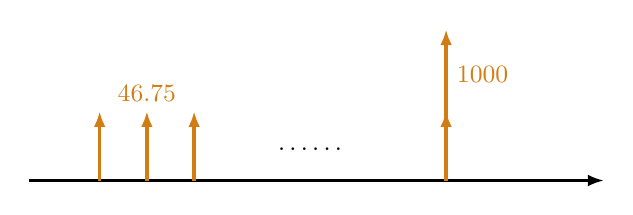
\begin{tikzpicture}[yscale=0.8]
  \draw[-{Latex[length=2mm]},thick] (-0.3,0) -- (7,0);
  \foreach \x in {0.6,1.2,1.8} {\up{\x}{1.1}{}}
  \node[above,posflow] at (1.2,1.1){\small $46.75$};
  \node at (3.3,0.5){\small \dots\dots};
  \up{5}{1.1}{}
  \draw[-{Latex[length=2mm]},very thick,posflow] (5,0) -- (5,2.4) node[right,pos=0.7]{\small 1000};
\end{tikzpicture}
\caption*{A bond pays periodic coupons ($A$) plus the face value ($F$) at maturity.}
\end{figure}

Here $y$ is the \term{yield}: it reflects the time value of money for the bond
payments, and $i^{*} = y/m$.

\begin{genform}
\[
P = A\,(P/A,\ i^{*},\ N) + F\,(P/F,\ i^{*},\ N),
\qquad A = \frac{r_c}{m}\,F,\qquad i^{*} = \frac{y}{m},\qquad N = Y\times m.
\]
\where{$P=$ bond price (today);\;
$F=$ face value (paid at maturity);\;
$A=$ coupon payment per period;\;
$r_c=$ coupon rate (annual);\;
$y=$ yield (annual);\;
$i^{*}=$ periodic yield;\;
$m=$ coupon payments per year;\;
$Y=$ years to maturity;\;
$N=$ total coupon periods.}
\end{genform}

\fillnote{What is $m$? It is the number of coupon periods per year, i.e.\ how
often the coupon is paid (and the yield compounded). So a bond that pays
semiannual coupons has $m=2$, and the per period rate used in the factors is
$i^{*}=y/m$.}

\textbf{If the yield gets higher, the price $P$ gets lower, because} the price is
just the present value of a fixed set of future cash flows (the coupons and the
face value). A higher yield discounts those future payments more heavily, so
each one is worth less today, and the total present value (the price) falls. This
is the standard inverse relationship between bond price and yield.

% ======================================================================
\section{Week Four: Risk, Portfolios, CAPM, and Arbitrage}
% ======================================================================

\textit{This part explains why we use CAPM (if you do not care, you can skip
straight to the formula).}

\subsection*{Financial risk and the need for a portfolio}
\term{Financial risk} is the uncertainty of the future pay off. But when you plot
the expected return against the volatility, there is no clear trend line.

\begin{figure}[h]
\centering
\begin{tabular}{cc}
\begin{minipage}{0.33\textwidth}
\centering
\small
\begin{tabular}{cc}
\toprule
Time Period ($t$) & Price ($P$)\\
\midrule
0 & 20\\ 1 & 21\\ 2 & 22\\ 3 & 20\\ 4 & 21\\
\bottomrule
\end{tabular}
\end{minipage}
&
\begin{minipage}{0.6\textwidth}
\centering
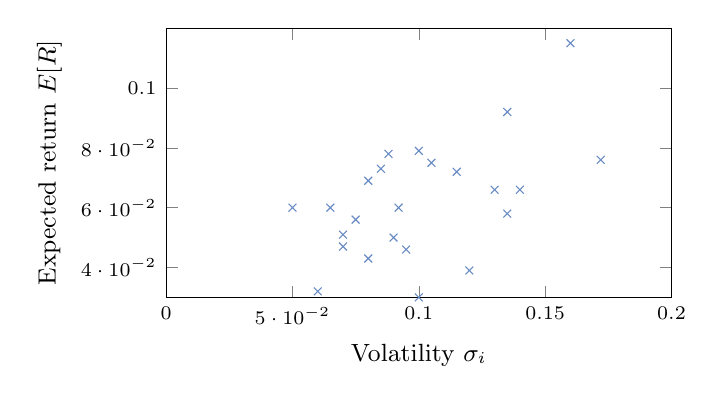
\begin{tikzpicture}
\begin{axis}[
  width=8cm,height=5cm,
  xlabel={\small Volatility $\sigma_i$}, ylabel={\small Expected return $E[R]$},
  xmin=0,xmax=0.2,ymin=0.03,ymax=0.12,
  xtick={0,0.05,0.1,0.15,0.2}, ytick={0.04,0.06,0.08,0.1},
  tick label style={font=\scriptsize},
]
\addplot[only marks,mark=x,negflow!70,mark size=2pt] coordinates{
(0.05,0.06)(0.06,0.032)(0.065,0.06)(0.07,0.047)(0.075,0.056)(0.08,0.069)
(0.085,0.073)(0.088,0.078)(0.09,0.05)(0.092,0.06)(0.095,0.046)(0.1,0.079)
(0.1,0.03)(0.105,0.075)(0.115,0.072)(0.12,0.039)(0.13,0.066)(0.135,0.058)
(0.14,0.066)(0.135,0.092)(0.16,0.115)(0.172,0.076)(0.08,0.043)(0.07,0.051)
};
\end{axis}
\end{tikzpicture}
\end{minipage}
\end{tabular}
\caption*{A price series (left) and the expected return vs.\ volatility cloud (right): no clear trend.}
\end{figure}

For the price data, the per period (log) return and its vector and variance are:
\[
P_{t_j} = P_{t_{j-1}}\,e^{\,r_{t_j}\Delta t},\qquad
r_{t_j} = \frac{1}{\Delta t}\ln\frac{P_{t_j}}{P_{t_{j-1}}},\qquad
\vec{R_i} = \begin{bmatrix} r_{t_1}\\ r_{t_2}\\ \vdots\\ r_{t_m}\end{bmatrix},\qquad
\sigma_i^{2} = \mathrm{Var}(\vec{R_i}).
\]

\subsection*{Modern Portfolio Theory (MPT)}
So we use \term{MPT}: we want to maximize our return while minimizing the
volatility. Assume we can invest our wealth by an amount $x_i$ in the $i$-th
asset. The expected return equals the weighted sum of the stocks we invested in,
while the portfolio volatility is defined through the covariance matrix:
\[
\vec{X} = \begin{bmatrix} x_1\\ x_2\\ \vdots\\ x_n\end{bmatrix},\qquad
\Sigma = \begin{bmatrix}
\sigma_{11} & \sigma_{12} & \cdots & \sigma_{1n}\\
\sigma_{21} & \sigma_{22} & \cdots & \sigma_{2n}\\
\vdots & \vdots & \ddots & \vdots\\
\sigma_{n1} & \sigma_{n2} & \cdots & \sigma_{nn}
\end{bmatrix},
\]
where $\sigma_{ii} = \mathrm{Var}(\vec{R_i})$ and
$\sigma_{ij} = \sigma_{ji} = \mathrm{Cov}(\vec{R_i}, \vec{R_j})$. Then
\[
\sigma_p = \sqrt{\vec{X}^{T}\Sigma\vec{X}},\qquad
\text{optimize: maximize } \mathbb{E}\!\left[\vec{R_p}\right] \text{ for a given } \sigma_p.
\]

We solve for $X$ by maximizing the expected return of the portfolio
$\mathbb{E}[R_p]$ for a given $\sigma_p$, which leads to CAPM. CAPM has a lot of
limitations but gives us a weighted estimate of the price of risk.

\subsection*{Efficiency frontier}
Using the assumptions and optimizing the expected return, we can create a
portfolio of stocks for any given portfolio volatility, which leads to an
\term{efficiency frontier}.

\fillnote{What is the ``high side''? For a given level of volatility there are two
portfolios on the boundary, one with a high return and one with a low return.
Only the upper (high return) half of the curve is interesting to us, because for
the same risk you would always prefer the higher return. The lower half is
dominated, so people mean the upper branch when they say ``efficient frontier''.}

\begin{figure}[h]
\centering
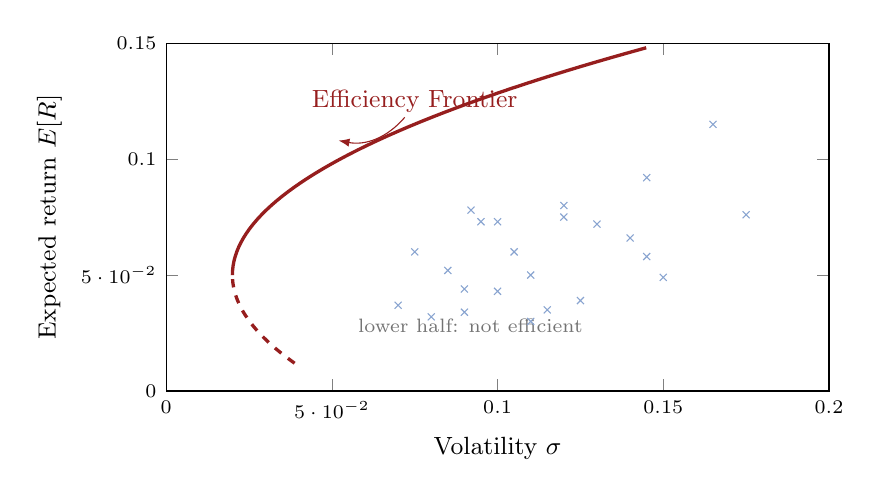
\begin{tikzpicture}
\begin{axis}[
  width=10cm,height=6cm,
  xlabel={\small Volatility $\sigma$}, ylabel={\small Expected return $E[R]$},
  xmin=0,xmax=0.2,ymin=0,ymax=0.15,
  xtick={0,0.05,0.1,0.15,0.2}, ytick={0,0.05,0.1,0.15},
  tick label style={font=\scriptsize},
]
\addplot[only marks,mark=x,negflow!55,mark size=1.8pt] coordinates{
(0.07,0.037)(0.08,0.032)(0.075,0.06)(0.09,0.044)(0.085,0.052)(0.1,0.073)
(0.095,0.073)(0.092,0.078)(0.11,0.05)(0.105,0.06)(0.1,0.043)(0.12,0.08)
(0.11,0.03)(0.12,0.075)(0.13,0.072)(0.125,0.039)(0.14,0.066)(0.145,0.058)
(0.15,0.049)(0.145,0.092)(0.165,0.115)(0.175,0.076)(0.09,0.034)(0.115,0.035)
};
% efficiency frontier: a Markowitz bullet (sideways parabola, nose at left)
\addplot[accent,very thick,domain=0.05:0.148,samples=50] ({0.02+13*(x-0.05)^2},{x});
\addplot[accent,very thick,dashed,domain=0.012:0.05,samples=25] ({0.02+13*(x-0.05)^2},{x});
\node[accent] at (axis cs:0.075,0.125){\small Efficiency Frontier};
\draw[accent,-{Latex[length=1.4mm]},thin] (axis cs:0.072,0.118) to[bend left] (axis cs:0.052,0.108);
\node[black!55,font=\scriptsize,anchor=west] at (axis cs:0.055,0.028){lower half: not efficient};
\end{axis}
\end{tikzpicture}
\caption*{The frontier is the left boundary of what portfolios can reach. Only the solid upper branch (the ``high side'') is efficient; the dashed lower branch is dominated.}
\end{figure}

\subsection*{Capital Market Line}
If it is possible to borrow or invest at the risk free rate, we can draw a
tangent line that intersects the $y$ axis at the risk free rate (the risk free
rate has a volatility of 0).
\begin{itemize}[nosep]
  \item Where it touches the frontier: the \term{tangency portfolio} /
        \term{market portfolio}.
  \item The tangent itself: the \term{Capital Market Line (CML)}.
\end{itemize}
If you invest, you should expect your result to lie on this line.

\begin{figure}[h]
\centering
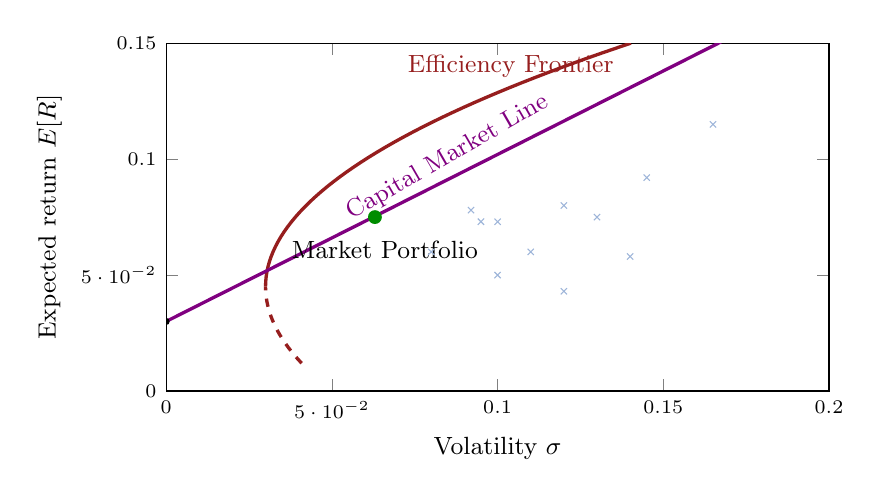
\begin{tikzpicture}
\begin{axis}[
  width=10cm,height=6cm,
  xlabel={\small Volatility $\sigma$}, ylabel={\small Expected return $E[R]$},
  xmin=0,xmax=0.2,ymin=0,ymax=0.15,
  xtick={0,0.05,0.1,0.15,0.2}, ytick={0,0.05,0.1,0.15},
  tick label style={font=\scriptsize},
]
\addplot[only marks,mark=x,negflow!45,mark size=1.6pt] coordinates{
(0.08,0.06)(0.1,0.073)(0.095,0.073)(0.092,0.078)(0.11,0.06)(0.12,0.08)
(0.13,0.075)(0.145,0.092)(0.165,0.115)(0.1,0.05)(0.12,0.043)(0.14,0.058)
};
% frontier
\addplot[accent,very thick,domain=0.045:0.15,samples=50] ({0.03+10*(x-0.045)^2},{x});
\addplot[accent,very thick,dashed,domain=0.012:0.045,samples=20] ({0.03+10*(x-0.045)^2},{x});
% CML tangent from rf=0.03
\addplot[violet,very thick,domain=0:0.2] {0.03 + 0.72*x};
\node[accent,anchor=west] at (axis cs:0.07,0.14){\small Efficiency Frontier};
\node[violet,rotate=30,anchor=south] at (axis cs:0.088,0.093){\small Capital Market Line};
\fill[green!55!black] (axis cs:0.063,0.075) circle (2.5pt);
\node[anchor=north] at (axis cs:0.066,0.069){\small Market Portfolio};
\node[anchor=east] at (axis cs:0,0.03){\small $r_f$};
\fill (axis cs:0,0.03) circle (1.3pt);
\end{axis}
\end{tikzpicture}
\caption*{The CML runs from $r_f$ (on the $y$ axis) and just touches the frontier at the market portfolio.}
\end{figure}

\textbf{Worked example (leverage along the CML).}
\fillnote{This is the example that was hard to read on the slide, explained step
by step.}

Suppose the market portfolio has an expected return of 7\% and the risk free
rate is $r_f = 3\%$. You have \$100 of your own money, but instead of just buying
the market portfolio you \emph{leverage up}:
\begin{itemize}[nosep]
  \item Invest your \$100 in the market portfolio (MP).
  \item Borrow another \$50 at the risk free rate $r_f$ and invest that in the MP
        as well.
\end{itemize}
Now you hold \$150 of the MP but only \$100 is yours, so you have leveraged up
along the CML by a factor of $150/100 = 1.5$. Both the risk and the extra return
scale by that same factor:
\[
\sigma_p = 1.5 \times \sigma_{mp} = 1.5 \times 0.06 = 0.09,
\qquad
\mathbb{E}[R_p] = 1.5\,(7\% - 3\%) + 3\% = 9\%.
\]
So by borrowing at $r_f$ and overinvesting in the market, you move up and to the
right along the CML: more volatility (0.09 instead of 0.06) in exchange for more
expected return (9\% instead of 7\%).

\begin{genform}
\[
\sigma_p = L\,\sigma_{mp},\qquad
\mathbb{E}[R_p] = L\big(\mathbb{E}[R_{mp}] - r_f\big) + r_f,\qquad
L = \frac{\text{total invested}}{\text{own money}}.
\]
\where{$L=$ leverage factor ($L>1$ means you borrowed, $L<1$ means you also hold
some risk free asset);\;
$\sigma_{mp}=$ volatility of the market portfolio;\;
$\mathbb{E}[R_{mp}]=$ expected return of the market portfolio;\;
$r_f=$ risk free rate.}
\end{genform}

\subsection*{CAPM}
\begin{itemize}[nosep]
  \item \term{MP} (market portfolio): represents the whole market.
  \item An asset has both \term{systematic} risk (associated with the market as a
        whole) and \term{idiosyncratic} risk (particular to the company).
  \item The market risk is designated by beta.
\end{itemize}
\[
\mathbb{E}[R_i] = r_f + \beta_i\big(\mathbb{E}[R_{MP}] - r_f\big),
\qquad
\beta_i = \frac{\sigma_{i,MP}}{\sigma_{MP}^{2}}
        = \frac{\rho_{i,MP}\,\sigma_i}{\sigma_{MP}}.
\]

\begin{genform}
\[
\mathbb{E}[R_i] = r_f + \beta_i\big(\mathbb{E}[R_{MP}] - r_f\big),
\qquad
\beta_i = \frac{\sigma_{i,MP}}{\sigma_{MP}^{2}} = \frac{\rho_{i,MP}\,\sigma_i}{\sigma_{MP}}.
\]
\where{$\mathbb{E}[R_i]=$ expected return the asset should earn;\;
$r_f=$ risk free rate (return for taking no risk);\;
$\mathbb{E}[R_{MP}]=$ expected return of the whole market;\;
$\big(\mathbb{E}[R_{MP}]-r_f\big)=$ market risk premium (extra return the market
pays for its risk);\;
$\beta_i=$ how much of that market risk the asset carries
($\beta=1$ moves with the market, $\beta>1$ more volatile, $\beta<1$ less);\;
$\sigma_{i,MP}=$ covariance of the asset with the market;\;
$\sigma_{MP}^{2}=$ market variance;\;
$\rho_{i,MP}=$ correlation of the asset with the market.}
\end{genform}

In words, the company return is
\[
R_{C,t} = \alpha_C + \beta_C' R_{MP,t} + \varepsilon_{C,t}.
\]
Volatility in $R_{MP,t}$ is systematic (``market'') risk; volatility in
$\varepsilon_{C,t}$ is idiosyncratic (``firm specific'') risk. Investors can use
portfolios to ``diversify away'' idiosyncratic risk, therefore there is no
``value'' to idiosyncratic risk. CAPM then says
\[
\mathbb{E}[R_C] = r_f + \beta_C\big(\mathbb{E}[R_{MP}] - r_f\big),
\]
where $\beta_C$ is a measure of risk for the company.

\begin{figure}[h]
\centering
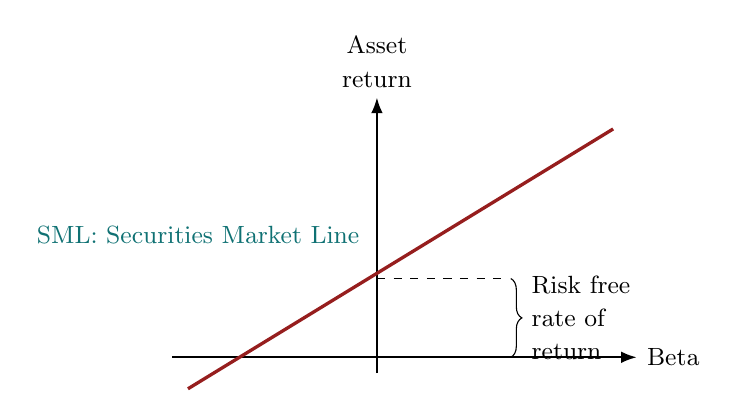
\begin{tikzpicture}
  \draw[-{Latex[length=2mm]},thick] (0,-0.2) -- (0,3.3) node[above,align=center]{\small Asset\\\small return};
  \draw[-{Latex[length=2mm]},thick] (-2.6,0) -- (3.3,0) node[right]{\small Beta};
  \draw[very thick,accent] (-2.4,-0.4) -- (3,2.9);
  \draw[dashed] (0,1.0) -- (1.6,1.0);
  \draw[decorate,decoration={brace,amplitude=4pt}] (1.7,1.0) -- (1.7,0)
        node[midway,right=4pt,align=left]{\small Risk free\\\small rate of\\\small return};
  \node[anchor=east,cTerm] at (-0.1,1.55){\small SML: Securities Market Line};
\end{tikzpicture}
\caption*{The Securities Market Line: intercept at $r_f$, slope set by the market risk premium.}
\end{figure}

\subsubsection*{Example: Estimating future stock price}
\textit{If asked for a future price, since we are already using CAPM (which
carries a lot of error), you can use either a continuous or an effective rate;
either way is fine.}

A company with a beta of 0.9 has a stock price currently trading at \$170 a
share. The current risk free rate is 2\%, and the market rate is 7\%. What is the
expected price of a share 5 years from now, if the company pays no dividends?
\[
\mathbb{E}[R_C] = r_f + \beta_C\big(\mathbb{E}[R_{MP}] - r_f\big)
= 2\% + 0.9(7\% - 2\%) = 6.5\%.
\]
\[
P_t = P_0\,e^{R_C\, t}
\quad\Longrightarrow\quad
P_5 = \$170\,e^{\,0.065 \times 5} = \$235.
\]

\begin{genform}
\[
\mathbb{E}[R_C] = r_f + \beta_C\big(\mathbb{E}[R_{MP}] - r_f\big),
\qquad
P_t = P_0\,e^{\,\mathbb{E}[R_C]\,t}.
\]
\where{$P_0=$ current share price;\;
$P_t=$ expected share price at time $t$;\;
$t=$ number of years ahead;\;
$\beta_C=$ company beta;\;
$\mathbb{E}[R_C]=$ the return demanded by CAPM, used as the growth rate of the
price (continuous form shown; the effective form $P_t=P_0(1+\mathbb{E}[R_C])^{t}$
works too).}
\end{genform}

\subsubsection*{Example: Dividend paying stock}
$P = \$10$, dividend $= \$0.10$ (quarterly), $\mathbb{E}[R_{MP}] = 10\%$,
$r_f = 3\%$, $\beta = 1.2$, find $P_3$.
\[
\mathbb{E}[R_C] = 3\% + 1.2(10\% - 3\%) = 11.4\%.
\]
Convert to a quarterly company rate:
\[
(1 + R_{C,q})^{4} = (1 + 11.4\%)\quad\Longrightarrow\quad R_{C,q} = 2.736\%.
\]
Cash flow: \$10 out today, \$0.10 each quarter for 12 quarters, and sell for
$P_3$ at the end of year 3:
\[
\$10 = \$0.10\,(P/A,\ 2.736\%,\ 12) + P_3\,(P/F,\ 11.4\%,\ 3)
\quad\Longrightarrow\quad P_3 = \$12.43.
\]
\begin{figure}[h]
\centering
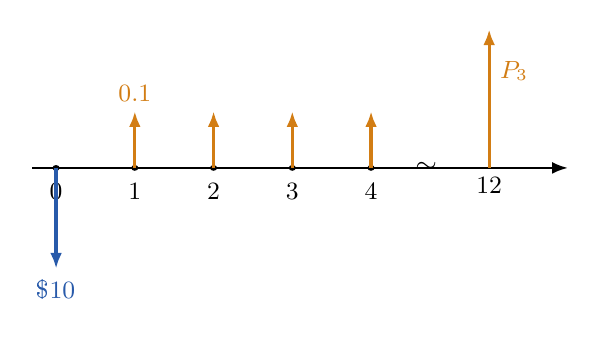
\begin{tikzpicture}[yscale=0.8]
  \draw[-{Latex[length=2mm]},thick] (-0.3,0) -- (6.5,0);
  \foreach \x/\n in {0/0,1/1,2/2,3/3,4/4} {\tick{\x}{\n}}
  \node at (4.7,0){$\sim$};
  \foreach \x in {1,2,3,4} {\up{\x}{0.9}{}}
  \node[above,posflow] at (1,0.9){\small 0.1};
  \draw[-{Latex[length=2mm]},very thick,posflow] (5.5,0) -- (5.5,2.2) node[right,pos=0.7]{\small $P_3$};
  \node[below] at (5.5,0){\small 12};
  \dn{0}{1.6}{\$10}
\end{tikzpicture}
\caption*{Dividends come in each quarter, the resale price $P_3$ at the end, and \$10 is paid today.}
\end{figure}

\begin{genform}
\[
P_0 = D\,(P/A,\ i_q,\ n) + P_T\,(P/F,\ \mathbb{E}[R_C],\ T),
\qquad (1+i_q)^{m} = 1 + \mathbb{E}[R_C].
\]
\where{$P_0=$ price paid today;\;
$D=$ dividend per period;\;
$n=$ number of dividend periods;\;
$i_q=$ per period (e.g.\ quarterly) company rate;\;
$m=$ periods per year;\;
$\mathbb{E}[R_C]=$ annual CAPM return;\;
$P_T=$ resale price after $T$ years.}
\end{genform}

\subsection*{Arbitrage}
In financial markets: \term{arbitrage} is the practice of taking advantage of a
price difference between two or more markets. Academic use: arbitrage occurs when
there is an opportunity to achieve a risk free gain at a rate greater than the
risk free rate. Fundamental to finance theory is the \term{no arbitrage
assumption} (``no free lunch''). It works well in theory but not always in the
real world.

\subsubsection*{Arbitrage Example}
Say you could buy a bushel of corn for \$10 today and enter into a forward
contract to deliver the corn for an agreed price of \$12 per bushel one year from
now (assume it costs you nothing to store the corn). Say you could also borrow at
10\%. What would you do?

Strategy (net \$0 today):
\begin{itemize}[nosep]
  \item Borrow \$10$x$.
  \item Buy $x$ bushels for \$10$x$.
\end{itemize}
\begin{figure}[h]
\centering
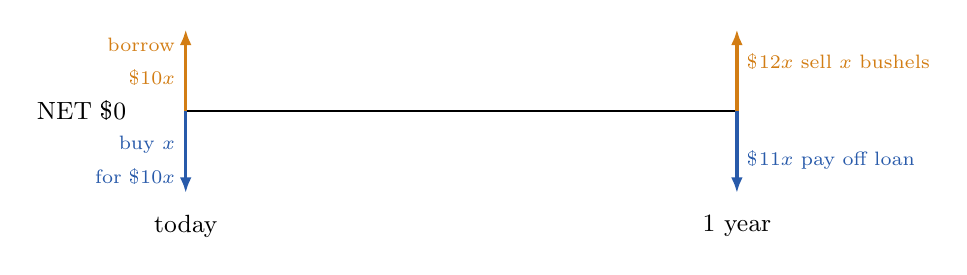
\begin{tikzpicture}[yscale=0.8]
  \draw[thick] (0,0) -- (7,0);
  \draw[-{Latex[length=2mm]},very thick,posflow] (0,0) -- (0,1.3) node[left,pos=0.6,align=right]{\scriptsize borrow\\\scriptsize \$10$x$};
  \draw[-{Latex[length=2mm]},very thick,negflow] (0,0) -- (0,-1.3) node[left,pos=0.6,align=right]{\scriptsize buy $x$\\\scriptsize for \$10$x$};
  \node[left=18pt] at (0,0){\small NET \$0};
  \node[below] at (0,-1.5){\small today};
  \draw[-{Latex[length=2mm]},very thick,posflow] (7,0) -- (7,1.3) node[right,pos=0.6]{\scriptsize \$12$x$ sell $x$ bushels};
  \draw[-{Latex[length=2mm]},very thick,negflow] (7,0) -- (7,-1.3) node[right,pos=0.6]{\scriptsize \$11$x$ pay off loan};
  \node[below] at (7,-1.5){\small 1 year};
\end{tikzpicture}
\caption*{Borrow and buy today (net \$0), then in one year sell at \$12$x$ and repay \$11$x$, keeping \$1$x$.}
\end{figure}

In one year you sell for \$12$x$ and repay \$11$x$, so you keep \$1$x$ at no risk.
As $x \to \infty$ this gives infinite profit. As demand for bushels today
increases, the price will increase until there is no arbitrage. The no arbitrage
price is
\[
\frac{\$12}{1 + 10\%} = \$10.91.
\]

\begin{genform}
\[
S_0 = \frac{F}{1 + r},\qquad\text{equivalently}\qquad F = S_0\,(1+r).
\]
\where{$S_0=$ fair spot (today) price with no arbitrage;\;
$F=$ agreed forward price;\;
$r=$ financing (borrowing) rate over the period.
If the real spot price is below $S_0$, you can borrow, buy, and lock in a risk
free profit.}
\end{genform}

\subsection*{Interest rate forwards}
In this course we treat futures $=$ forwards. At a given interest rate curve, the
forward rate $r_{t_1,t_2}$ is the appropriate rate between $t_1$ and $t_2$:
\[
r_{1,2} = \frac{r_{0,2}\,t_2 - r_{0,1}\,t_1}{t_2 - t_1}.
\]
\begin{figure}[h]
\centering
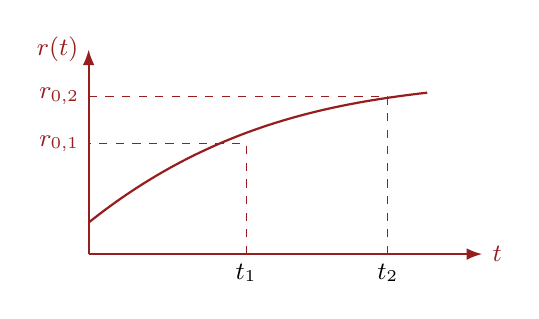
\begin{tikzpicture}[scale=1]
  \draw[-{Latex[length=2mm]},thick,accent] (0,0) -- (5,0) node[right]{\small $t$};
  \draw[-{Latex[length=2mm]},thick,accent] (0,0) -- (0,2.6) node[left]{\small $r(t)$};
  \draw[accent,thick] (0,0.4) .. controls (1.5,1.6) and (3,1.9) .. (4.3,2.05);
  \draw[dashed,accent] (2,0) -- (2,1.4) -- (0,1.4) node[left]{\small $r_{0,1}$};
  \draw[dashed,accent] (3.8,0) -- (3.8,2.0) -- (0,2.0) node[left]{\small $r_{0,2}$};
  \node[below] at (2,0){\small $t_1$};
  \node[below] at (3.8,0){\small $t_2$};
\end{tikzpicture}
\caption*{A rising interest rate curve, with the spot rates $r_{0,1}$ and $r_{0,2}$ marked.}
\end{figure}

\begin{genform}
\[
r_{t_1,t_2} = \frac{r_{0,t_2}\,t_2 - r_{0,t_1}\,t_1}{t_2 - t_1}.
\]
\where{$r_{0,t}=$ spot rate from today out to time $t$ (read off the curve);\;
$r_{t_1,t_2}=$ forward rate that applies between $t_1$ and $t_2$;\;
$t_1,t_2=$ the two times.}
\end{genform}

\subsubsection*{Foreign Exchange Example}
Canadian risk free rate is 3\%, US risk free rate is 2.5\%, current FX $= 0.9$
US\$/C\$. What would be a fair FX rate one year from now that you would commit to
today (the one year forward FX rate)?

Grow \$1 CAD at 3\% and \$0.90 USD at 2.5\%, then take the ratio:
\[
\text{C\$}1 \to \text{C\$}1.03, \qquad \text{US\$}0.90(1+0.025) = \text{US\$}0.9225,
\]
\[
FX_1 = \frac{\text{US\$}0.9225}{\text{C\$}1.03} = 0.896\ \text{US\$/C\$}.
\]
\begin{figure}[h]
\centering
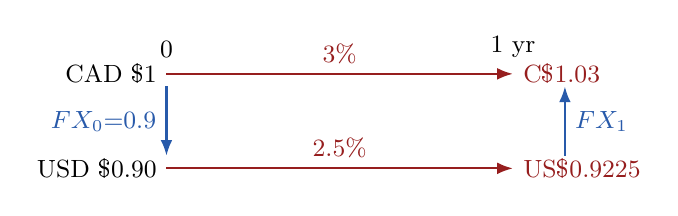
\begin{tikzpicture}[yscale=0.8,xscale=1.1]
  \node[left] at (0,1.5){\small CAD \$1};
  \node[left] at (0,0){\small USD \$0.90};
  \draw[-{Latex[length=2mm]},accent,thick] (0,1.5) -- (4,1.5) node[midway,above]{\small 3\%} node[right]{\small C\$1.03};
  \draw[-{Latex[length=2mm]},accent,thick] (0,0) -- (4,0) node[midway,above]{\small 2.5\%} node[right]{\small US\$0.9225};
  \draw[-{Latex[length=2mm]},negflow,thick] (0,1.3) -- (0,0.2) node[midway,left]{\small $FX_0{=}0.9$};
  \draw[-{Latex[length=2mm]},negflow,thick] (4.6,0.2) -- (4.6,1.3) node[midway,right]{\small $FX_1$};
  \node[above] at (0,1.6){\small 0}; \node[above] at (4,1.6){\small 1 yr};
\end{tikzpicture}
\caption*{Grow each currency at its own risk free rate, then take the ratio to get the forward rate.}
\end{figure}

\begin{genform}
\[
FX_1 = FX_0\,\frac{1 + r_{\text{quote}}}{1 + r_{\text{base}}}.
\]
\where{$FX$ is quoted as (quote currency) per (base currency), here US\$ per C\$;\;
$FX_0=$ current (spot) exchange rate;\;
$FX_1=$ one year forward rate;\;
$r_{\text{base}}=$ risk free rate of the base currency (C\$);\;
$r_{\text{quote}}=$ risk free rate of the quote currency (US\$).}
\end{genform}

\subsection*{Replicating a project with the market}
Project payoff is \$140 if the market goes up and \$30 if the market goes down.
The risk free rate is 5\% for this period. The current MP is priced at \$100. If
the market goes up it will be worth \$120; if it goes down it will be worth \$95.

We know the market portfolio (which can go up and down) and we know the project,
but not $P$ (the current price). The risk free asset is risk free, so either way
it returns 1.05.

\begin{figure}[h]
\centering
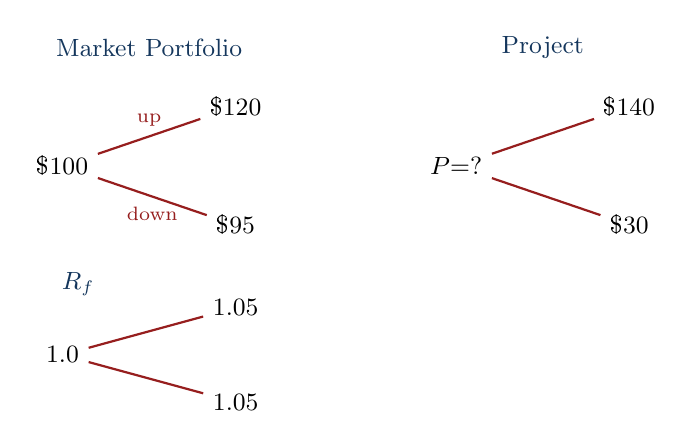
\begin{tikzpicture}[yscale=0.75,xscale=1.0]
  \node (a) at (0,0){\small \$100};
  \node (au) at (2.2,1){\small \$120};
  \node (ad) at (2.2,-1){\small \$95};
  \draw[accent,thick] (a)--(au) node[midway,above]{\scriptsize up};
  \draw[accent,thick] (a)--(ad) node[midway,below]{\scriptsize down};
  \node[cHead] at (1.1,2){\small Market Portfolio};
  \node (b) at (5,0){\small $P{=}?$};
  \node (bu) at (7.2,1){\small \$140};
  \node (bd) at (7.2,-1){\small \$30};
  \draw[accent,thick] (b)--(bu);
  \draw[accent,thick] (b)--(bd);
  \node[cHead] at (6.1,2){\small Project};
  \node (c) at (0,-3.2){\small 1.0};
  \node (cu) at (2.2,-2.4){\small 1.05};
  \node (cd) at (2.2,-4){\small 1.05};
  \draw[accent,thick] (c)--(cu);
  \draw[accent,thick] (c)--(cd);
  \node[cHead] at (0.2,-2){\small $R_f$};
\end{tikzpicture}
\caption*{The market, the project, and the risk free asset as single step trees.}
\end{figure}

We replicate the project with $a$ units of the MP and $b$ units of the risk free
asset ($a \sim MP$, $b \sim R_f$):
\[
\begin{cases}
\text{up:} & \$120\,a + \$1.05\,b = \$140,\\[2pt]
\text{down:} & \$95\,a + \$1.05\,b = \$30.
\end{cases}
\quad\Longrightarrow\quad a = 4.4,\quad b = -369.53.
\]
Therefore the no arbitrage price is
\[
P = \$100 \times 4.4 - \$1 \times 369.53 = \$70.48.
\]

\begin{genform}
\[
\begin{cases}
MP_u\,a + R_f\,b = X_u,\\[2pt]
MP_d\,a + R_f\,b = X_d,
\end{cases}
\qquad\Longrightarrow\qquad
P = MP_0\,a + b.
\]
\where{$a=$ units of the market portfolio in the replicating portfolio;\;
$b=$ dollars placed in the risk free asset ($b<0$ means borrowing);\;
$MP_0=$ current market price;\;
$MP_u,MP_d=$ market value in the up / down state;\;
$R_f = 1+r_f$;\;
$X_u,X_d=$ project payoff in the up / down state;\;
$P=$ the replicating cost, i.e.\ the no arbitrage price of the project.}
\end{genform}

\textbf{Using probabilities.}
In the replication above we did not use the probability of the market going up or
down. If the probability of the market going up is 60\%, what is the expected
return of the MP?
\[
\mathbb{E}[R_{MP}] = \frac{\mathbb{E}[\text{payoff}_{MP}]}{\text{price}_{MP}} - 1
= \frac{\$120 \times 60\% + \$95 \times 40\%}{\$100} - 1 = 10\%.
\]
And for the project:
\[
\mathbb{E}[R_{proj}] = \frac{\$140 \times 60\% + \$30 \times 40\%}{\$70.48} - 1 = 36.2\%.
\]
We can then use CAPM to find the beta of the project:
\[
\mathbb{E}[R_{proj}] = r_f + \beta_{proj}\big(\mathbb{E}[R_{MP}] - r_f\big),\qquad
36.2\% = 5\% + \beta_{proj}(10\% - 5\%)\ \Longrightarrow\ \beta_{proj} = 6.24.
\]

\textbf{What if the expected payoff of the project were \$140 regardless of the
market?}
\[
\frac{\$140}{1.05} = \$133.
\]
What if the project payoff had a 50\% chance of being \$150 and a 50\% chance of
being \$130?
\[
\mathbb{E}[\text{payoff}] = \$150 \times 50\% + \$130 \times 50\% = \$140.
\]
For the 50/50 case, since there is no correlation with the market the beta is 0,
so the price is the same as above, \$133.

\subsection*{Investments with systematic and idiosyncratic risk}
\begin{itemize}[nosep]
  \item If the market goes up: 60\% chance the payoff is \$80k, otherwise \$50k.
  \item If the market goes down: 60\% chance the payoff is \$55k, otherwise \$20k.
  \item Current market portfolio is \$45 (up $\to$ \$60, down $\to$ \$40).
  \item Risk free rate is 5\%.
  \item An initial investment of \$20k is required for R\&D; determine the maximum
        price for the project.
\end{itemize}

\begin{figure}[h]
\centering
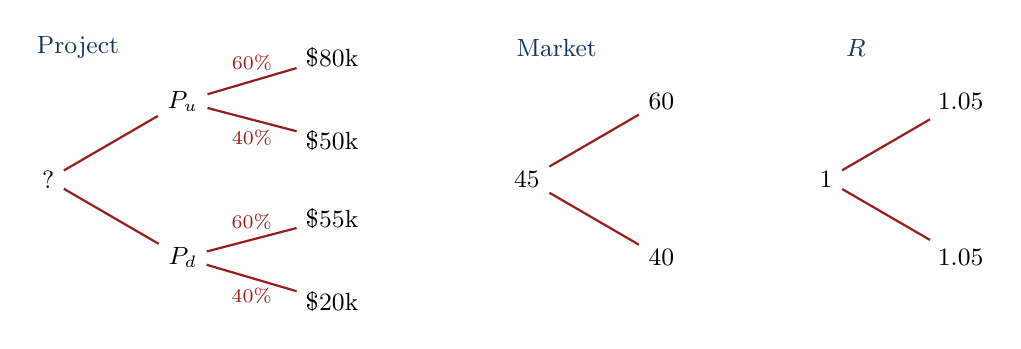
\begin{tikzpicture}[yscale=0.62,xscale=0.95]
  \node (q) at (0,0){\small ?};
  \node (pu) at (1.8,1.6){\small $P_u$};
  \node (pd) at (1.8,-1.6){\small $P_d$};
  \draw[accent,thick] (q)--(pu);
  \draw[accent,thick] (q)--(pd);
  \node (u1) at (3.8,2.5){\small \$80k};
  \node (u2) at (3.8,0.8){\small \$50k};
  \draw[accent,thick] (pu)--(u1) node[midway,above]{\scriptsize 60\%};
  \draw[accent,thick] (pu)--(u2) node[midway,below]{\scriptsize 40\%};
  \node (d1) at (3.8,-0.8){\small \$55k};
  \node (d2) at (3.8,-2.5){\small \$20k};
  \draw[accent,thick] (pd)--(d1) node[midway,above]{\scriptsize 60\%};
  \draw[accent,thick] (pd)--(d2) node[midway,below]{\scriptsize 40\%};
  \node[cHead] at (0.4,2.7){\small Project};
  \node (m) at (6.4,0){\small 45};
  \node (mu) at (8.2,1.6){\small 60};
  \node (md) at (8.2,-1.6){\small 40};
  \draw[accent,thick] (m)--(mu);
  \draw[accent,thick] (m)--(md);
  \node[cHead] at (6.8,2.7){\small Market};
  \node (r) at (10.4,0){\small 1};
  \node (ru) at (12.2,1.6){\small 1.05};
  \node (rd) at (12.2,-1.6){\small 1.05};
  \draw[accent,thick] (r)--(ru);
  \draw[accent,thick] (r)--(rd);
  \node[cHead] at (10.8,2.7){\small $R$};
\end{tikzpicture}
\caption*{The project has a two level tree: first the market (systematic), then the firm specific (idiosyncratic) branch.}
\end{figure}

First collapse the idiosyncratic branches into expected payoffs in each market
state:
\[
\mathbb{E}[P_u] = 0.6 \times 80\text{k} + 0.4 \times 50\text{k} = 68\text{k},\qquad
\mathbb{E}[P_d] = 0.6 \times 55\text{k} + 0.4 \times 20\text{k} = 41\text{k}.
\]
Now replicate with $a$ (market) and $b$ (risk free):
\[
\begin{cases}
a(60) + b(1.05) = 68\text{k},\\[2pt]
a(40) + b(1.05) = 41\text{k},
\end{cases}
\quad\Longrightarrow\quad a = 1.35\text{k},\quad b = -12.38\text{k}.
\]
Therefore
\[
P_0 = 1.35\text{k} \times 45 - 12.38\text{k} = 48.37\text{k}.
\]
However, since we need an initial investment of \$20k, we should buy the project
for \$28.37k or less (that is, $48.37\text{k} - 20\text{k}$).

\begin{genform}
\[
\mathbb{E}[P_u] = \textstyle\sum_k p_k\,X_{u,k},\quad
\mathbb{E}[P_d] = \textstyle\sum_k p_k\,X_{d,k},\quad
P_0 = MP_0\,a + b,\quad
P_{\max} = P_0 - I_0.
\]
\where{$X_{u,k},X_{d,k}=$ the idiosyncratic payoffs in the up / down market
state;\;
$p_k=$ their probabilities;\;
$\mathbb{E}[P_u],\mathbb{E}[P_d]=$ expected payoff once the firm specific risk is
averaged out;\;
$a,b=$ replicating amounts (market and risk free), solved as before;\;
$I_0=$ required initial investment (here the \$20k R\&D);\;
$P_{\max}=$ the most you should pay for the project.}
\end{genform}

\subsection*{Risky bond, accounting for default}
A company is looking to issue a 5 year bond with a coupon rate of 5\% paid
annually. The risk neutral probability of the company defaulting on any given
year is 5\%, and in the case of a default only half of the principal will be paid
out. What should be the price of the bond if the risk free rate is 3\%? What is
the yield rate?

Each year the bond either survives (95\%) and pays its \$5 coupon, or defaults
(5\%) and pays \$50 (half of \$100 principal). At maturity a surviving bond pays
$5 + 100$.

\begin{figure}[h]
\centering
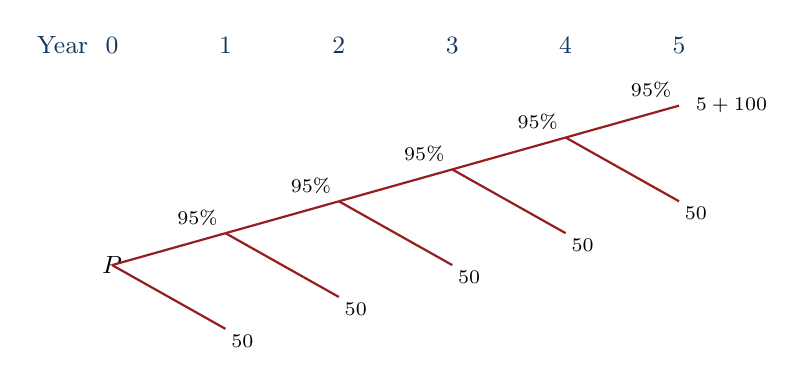
\begin{tikzpicture}[scale=0.9]
  \foreach \k/\x in {0/0,1/1.6,2/3.2,3/4.8,4/6.4,5/8.0}{\node[cHead] at (\x,3.1){\small \k};}
  \node[left,cHead] at (-0.2,3.1){\small Year};
  \node (p) at (0,0){\small $P$};
  \foreach \i in {1,...,5}{
    \pgfmathsetmacro\xx{1.6*\i}
    \pgfmathsetmacro\xp{1.6*(\i-1)}
    \pgfmathsetmacro\yy{0.45*\i}
    \pgfmathsetmacro\yp{0.45*(\i-1)}
    \draw[accent,thick] (\xp,\yp) -- (\xx,\yy);
    \draw[accent,thick] (\xp,\yp) -- (\xx,{\yp-0.9});
    \node[above left=-1pt] at (\xx,\yy){\scriptsize 95\%};
    \node[below right=-2pt] at (\xx,{\yp-0.9}){\scriptsize 50};
  }
  \node[right] at (8.1,2.25){\scriptsize $5+100$};
\end{tikzpicture}
\caption*{Each year: survive (95\%) and pay the \$5 coupon, or default (5\%) and recover \$50.}
\end{figure}

Work backwards. The value in the up (survive) state at $t=4$ is:
\[
P^{(4)}_{up} = 5 + \frac{105 \times 95\% + 50 \times 5\%}{1.03} = 104.27,
\qquad P^{(4)}_{00} = 50 \;(\text{default state}).
\]
Then roll the same formula back through each earlier stage:
\[
P^{(3)}_{up} = 5 + \frac{95\% \times 104.27 + 50 \times 5\%}{1.03} = 103.60,
\]
\[
P^{(2)}_{up} = 5 + \frac{95\% \times 103.60 + 50 \times 5\%}{1.03} = 102.48,
\]
\[
P^{(1)}_{up} = 5 + \frac{95\% \times 102.48 + 50 \times 5\%}{1.03} = 102.41,
\]
\[
P_0 = \frac{102.41 \times 95\% + 50 \times 50\%}{1.03} = 96.88.
\]
Finally, find the yield:
\[
96.88 = 5\,(P/A, y, 5) + 100\,(P/F, y, 5)\quad\Longrightarrow\quad y = 5.735\%.
\]

\begin{genform}
\[
P^{(k)} = C + \frac{(1-p)\,P^{(k+1)} + p\,R}{1 + r_f},
\qquad
P_0 = C\,(P/A, y, N) + F\,(P/F, y, N).
\]
\where{$P^{(k)}=$ bond value in the surviving state at year $k$ (worked
backwards, with the maturity payment $C+F$ included at $k=N$);\;
$C=$ coupon payment;\;
$p=$ default probability per year;\;
$R=$ recovery if default (here half the principal);\;
$r_f=$ risk free rate;\;
$F=$ face value;\;
$y=$ yield, found by matching the price $P_0$ in the last equation.}
\end{genform}

% ======================================================================
\section{Week Five: Comparing Projects (Present Worth and Annual Worth)}
% ======================================================================

% alternative colours (match the lecture slides)
\definecolor{cHonda}{HTML}{B23A3A}
\definecolor{cTesla}{HTML}{2E6FB0}
\definecolor{cLexus}{HTML}{2E8B57}

\subsection*{Multiple projects (investments)}
\begin{enumerate}[nosep]
  \item \term{Independent:} make the decisions separately (project by project).
  \item \term{Mutually exclusive:} choosing one will exclude all the other
        options, therefore we need to choose the best one.
\end{enumerate}
\term{Related but not mutually exclusive:} form project combinations that are
mutually exclusive, then find the best combination.

\subsection*{What does a project cash flow look like}
\begin{itemize}[nosep]
  \item First we have the \term{first cost:} a one time cost at the beginning
        (car example: the money to buy the car).
  \item Then we have some revenues or savings (car example).
  \item \term{O\&M} (operation and maintenance): car insurance or fuel.
  \item \term{Salvage value:} selling the car.
\end{itemize}

Because time changes the value of money, we want to evaluate benefits against
costs at different times, i.e.\ evaluate if it is worth it, using a
\term{discount rate}.

\subsection*{MARR}
\term{MARR} is the minimum acceptable rate of return. It is usually estimated
from the rate of return of the best alternative (if I do not invest in this one,
what do I get if I put it somewhere else?). We want the project's return to be
more than MARR, and we assume you can always earn MARR on some other project.

\subsection*{Comparison methods}

\subsubsection*{1. Present Worth (PW)}
The \term{present worth} is the present value of the benefits minus costs,
discounted at MARR. It is the amount by which the project is beating the best
alternative, expressed in today's value.
\begin{itemize}[nosep]
  \item $PW > 0$: acceptable.
  \item $PW < 0$: not acceptable (this does not mean the project is unprofitable,
        but doing nothing is better).
\end{itemize}

\textbf{Example 1: Calculating PW.}
You are planning to purchase a Honda Civic that has a life of 10 years. MARR is
5\%. The annual benefits are worth \$4000, and the annual costs are worth \$1000.
The first cost is \$20{,}000, and the salvage value after 10 years is \$4000.
What is the PW of purchasing the Honda Civic?
\[
PW = -20{,}000 + (4000 - 1000)\,(P/A, 5\%, 10) + 4000\,(P/F, 5\%, 10) = 5621.
\]
\begin{figure}[h]
\centering
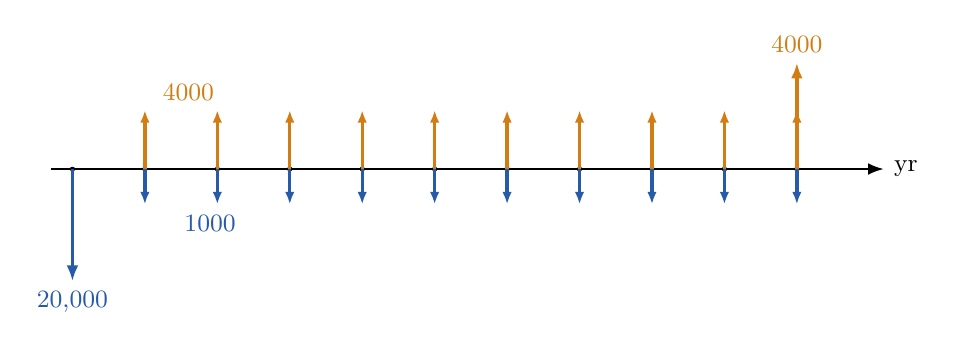
\begin{tikzpicture}[yscale=0.75,xscale=0.92]
  \draw[-{Latex[length=2mm]},thick] (-0.3,0) -- (11.2,0) node[right]{\small yr};
  \foreach \x in {0,...,10}{\fill (\x,0) circle (1.1pt);}
  \foreach \x in {1,...,10}{\draw[-{Latex[length=1.6mm]},very thick,posflow] (\x,0) -- (\x,1.0);}
  \foreach \x in {1,...,10}{\draw[-{Latex[length=1.6mm]},very thick,negflow] (\x,0) -- (\x,-0.6);}
  \draw[-{Latex[length=2mm]},very thick,posflow] (10,0) -- (10,1.8);
  \node[above,posflow] at (1.6,1.0){\small 4000};
  \node[below,negflow] at (1.9,-0.62){\small 1000};
  \node[above,posflow] at (10,1.8){\small 4000};
  \draw[-{Latex[length=2mm]},very thick,negflow] (0,0) -- (0,-1.9);
  \node[below,negflow] at (0,-1.9){\small 20{,}000};
\end{tikzpicture}
\caption*{Honda Civic: \$20{,}000 first cost at year 0, net \$3000 (benefit \$4000, cost \$1000) each year, and \$4000 salvage at year 10.}
\end{figure}

\begin{genform}
\[
PW = -FC + (B - C)\,(P/A, i, N) + S\,(P/F, i, N),
\qquad \text{accept if } PW > 0.
\]
\where{$FC=$ first cost (paid at year 0);\;
$B=$ annual benefit;\;
$C=$ annual cost;\;
$(B-C)=$ net annual cash flow;\;
$S=$ salvage value at the end;\;
$i=$ MARR;\;
$N=$ project life.}
\end{genform}

\subsubsection*{2. Annual Worth (AW)}
Same example, using \term{annual worth}: instead of collapsing everything to a
present value, spread it into an equivalent level amount per year.
\[
AW = -20{,}000\,(A/P, 5\%, 10) + 3000 + 4000\,(A/F, 5\%, 10) = 728.
\]
(Check: this is the same decision as PW, since $AW = PW\,(A/P, 5\%, 10)$, and
$5621\,(A/P,5\%,10) = 728$.)

\begin{genform}
\[
AW = -FC\,(A/P, i, N) + (B - C) + S\,(A/F, i, N) = PW\,(A/P, i, N),
\qquad \text{accept if } AW > 0.
\]
\where{same symbols as PW above;\;
the first cost is spread over the life with $(A/P)$, and the salvage is spread
with $(A/F)$. Because PW and AW differ only by the factor $(A/P, i, N)$, they
always give the same accept / reject decision.}
\end{genform}

\subsection*{Evaluating mutually exclusive projects}
Here we can only choose one best option. Four steps to use PW to evaluate
projects:
\begin{enumerate}[nosep]
  \item Define the time horizon.
  \item Develop the cash flows for each alternative.
  \item Calculate the PW using MARR.
  \item Compare the PWs and pick the best.
\end{enumerate}

\begin{genform}
\[
\text{choose the alternative } j^{\star} = \arg\max_{j} \; PW_j
\quad\text{(all compared over the same horizon, and } PW_{j^\star} > 0).
\]
\where{$PW_j=$ present worth of alternative $j$;\;
every alternative must be evaluated over the \emph{same} time horizon;\;
if the best PW is still negative, do nothing. AW works the same way, comparing
$AW_j$.}
\end{genform}

\subsubsection*{Example: same lives}
Choosing between two mutually exclusive options:

\begin{center}
\small
\begin{tabular}{lrr}
\toprule
 & \textcolor{cHonda}{\textbf{Honda Civic}} & \textcolor{cTesla}{\textbf{Tesla Model S}}\\
\midrule
FC & \textcolor{cHonda}{\$20{,}000} & \textcolor{cTesla}{\$100{,}000}\\
Annual benefit $-$ cost & \textcolor{cHonda}{\$3{,}000} & \textcolor{cTesla}{\$12{,}000}\\
Life & \textcolor{cHonda}{10 years} & \textcolor{cTesla}{10 years}\\
Salvage Value & \textcolor{cHonda}{\$4{,}000} & \textcolor{cTesla}{\$14{,}000}\\
MARR & \textcolor{cHonda}{5\%} & \textcolor{cTesla}{5\%}\\
\bottomrule
\end{tabular}
\end{center}

We calculated the Honda Civic already:
\begin{enumerate}[nosep]
  \item Both time horizons are 10 years.
  \item Compute each PW over those 10 years.
  \item $PW_{\text{Honda}} = 5621$.
\end{enumerate}
And for the Tesla:
\[
PW_{\text{Tesla}} = -100{,}000 + 12{,}000\,(P/A, 5\%, 10) + 14{,}000\,(P/F, 5\%, 10) = 1255.
\]
Since the Honda Civic has a higher present worth ($5621 > 1255$), we choose that.

\subsection*{What if the time horizon is different?}
Example: one toothbrush costs \$5 and lasts two years, another costs \$4 and
lasts one year. The two options cover different spans, so we cannot compare their
present worths directly. There are two ways to fix this.

\subsubsection*{Method 1: Repeated lives}
Assume the project repeats itself (e.g.\ you always need a car or a toothbrush).
Use the \term{Least Common Multiple (LCM)} of the individual lives as the study
horizon, then repeat each project's cash flow to fill that horizon.

\begin{figure}[h]
\centering
\begin{tikzpicture}[yscale=0.62,xscale=0.62]
  % top line: life 4, three cycles -> LCM 12
  \draw[-{Latex[length=2mm]},thick] (-0.3,0) -- (12.6,0);
  \foreach \c/\col in {0/posflow,4/accent,8/cHonda}{
    \draw[-{Latex[length=1.6mm]},very thick,negflow] (\c,0) -- (\c,-0.9);
    \foreach \k in {1,2,3,4}{\draw[-{Latex[length=1.6mm]},very thick,\col] (\c+\k,0) -- (\c+\k,{1.0+0.25*(\k==4)});}
  }
  \node[left] at (-0.4,0.6){\small Project A};
  % bottom line: life 3, four cycles -> LCM 12
  \begin{scope}[yshift=-3cm]
  \draw[-{Latex[length=2mm]},thick] (-0.3,0) -- (12.6,0);
  \foreach \c/\col in {0/posflow,3/accent,6/cHonda,9/cLexus}{
    \draw[-{Latex[length=1.6mm]},very thick,negflow] (\c,0) -- (\c,-0.9);
    \foreach \k in {1,2,3}{\draw[-{Latex[length=1.6mm]},very thick,\col] (\c+\k,0) -- (\c+\k,{1.0+0.25*(\k==3)});}
  }
  \node[left] at (-0.4,0.6){\small Project B};
  \end{scope}
\end{tikzpicture}
\caption*{Repeated lives: each project is repeated (a down arrow restarts each cycle, colours mark the cycles) until both reach the LCM of their lives.}
\end{figure}

\textbf{Example 2: PW with repeated lives.} Now compare the Honda Civic to a
Lexus RX.

\begin{center}
\small
\begin{tabular}{lrr}
\toprule
 & \textcolor{cHonda}{\textbf{Honda Civic}} & \textcolor{cLexus}{\textbf{Lexus RX}}\\
\midrule
FC & \textcolor{cHonda}{\$20{,}000} & \textcolor{cLexus}{\$40{,}000}\\
Annual benefit $-$ cost & \textcolor{cHonda}{\$3{,}000} & \textcolor{cLexus}{\$8{,}000}\\
Life & \textcolor{cHonda}{10 years} & \textcolor{cLexus}{\textbf{5 years}}\\
Salvage Value & \textcolor{cHonda}{\$4{,}000} & \textcolor{cLexus}{\$13{,}000}\\
MARR & \textcolor{cHonda}{5\%} & \textcolor{cLexus}{5\%}\\
\bottomrule
\end{tabular}
\end{center}

The LCM of 10 and 5 is 10 years. The Honda already spans 10 years ($PW = 5621$).
For the Lexus, work out one 5 year cycle, then repeat it once more (shifted 5
years into the future):
\[
PW_{\text{Lexus}}(5\text{ yr}) = -40{,}000 + 8000\,(P/A, i, 5) + 13{,}000\,(P/F, i, 5) = 4822,
\]
\[
PW_{\text{Lexus}}(10\text{ yr}) = 4822 + 4822\,(P/F, i, 5) = 8600.
\]
Now we see the Lexus has a higher PW ($8600 > 5621$), so we choose the Lexus.

\begin{figure}[h]
\centering
\begin{tikzpicture}[yscale=0.62,xscale=0.72]
  % Honda 10 yr
  \draw[-{Latex[length=2mm]},thick,cHonda] (-0.3,0) -- (11,0);
  \foreach \x in {1,...,10}{\draw[-{Latex[length=1.4mm]},very thick,cHonda] (\x,0) -- (\x,0.9);}
  \draw[-{Latex[length=1.8mm]},very thick,cHonda] (10,0) -- (10,1.6);
  \draw[-{Latex[length=1.8mm]},very thick,cHonda] (0,0) -- (0,-1.2);
  \node[cHonda,left] at (-0.4,-0.6){\small Honda};
  \node[cHonda,below] at (0,-1.2){\scriptsize 20k};
  \node[cHonda,above] at (1.6,0.9){\scriptsize 3000};
  \node[cHonda,above] at (10,1.6){\scriptsize 4000};
  % Lexus 5+5
  \begin{scope}[yshift=-2.8cm]
  \draw[-{Latex[length=2mm]},thick,cLexus] (-0.3,0) -- (11,0);
  \foreach \x in {1,...,10}{\draw[-{Latex[length=1.4mm]},very thick,cLexus] (\x,0) -- (\x,0.9);}
  \draw[-{Latex[length=1.8mm]},very thick,cLexus] (5,0) -- (5,1.6);
  \draw[-{Latex[length=1.8mm]},very thick,cLexus] (10,0) -- (10,1.6);
  \draw[-{Latex[length=1.8mm]},very thick,negflow] (0,0) -- (0,-1.2);
  \draw[-{Latex[length=1.8mm]},very thick,negflow] (5,0) -- (5,-1.2);
  \node[cLexus,left] at (-0.4,-0.6){\small Lexus};
  \node[negflow,below] at (0,-1.2){\scriptsize 40k};
  \node[negflow,below] at (5,-1.2){\scriptsize 40k};
  \node[cLexus,above] at (2,0.9){\scriptsize 8000};
  \node[cLexus,above] at (5,1.6){\scriptsize 13k};
  \node[cLexus,above] at (10,1.6){\scriptsize 13k};
  \end{scope}
\end{tikzpicture}
\caption*{Honda over 10 years vs.\ the Lexus repeated twice (buy again at year 5) to fill the same 10 year horizon.}
\end{figure}

We can also use \term{AW} for repeated lives. The nice thing about AW is that it
already annualizes, so you can compute each one over its \emph{own} life and
compare directly:
\[
AW_{\text{Honda}} = 728,\qquad
AW_{\text{Lexus}} = -40{,}000\,(A/P, 5\%, 5) + 8000 + 13{,}000\,(A/F, 5\%, 5) = 1114.
\]
Again the Lexus wins ($1114 > 728$), the same decision as PW.

\begin{genform}
\[
PW_{\text{LCM}} = PW_{\text{one life}}\sum_{k=0}^{n-1}(P/F, i, kN),
\qquad n = \frac{\text{LCM}}{N};
\qquad\text{or just compare } AW \text{ over each own life.}
\]
\where{$N=$ one project's life;\;
$\text{LCM}=$ least common multiple of all the lives (the common horizon);\;
$n=$ number of times the project repeats;\;
$PW_{\text{one life}}=$ present worth of a single cycle;\;
the AW route avoids the repetition entirely, because AW is already a per year
amount and does not change when the project repeats.}
\end{genform}

\subsubsection*{Method 2: Study period}
Instead of stretching to the LCM, pick a common \term{study period} and cut every
project off at the end of it. Here, if we terminate at the end of the shorter
life, we compare both over that same period. When we cut a longer project short,
we replace its salvage with an estimate of what it is worth at the end of the
study period (adjust $S$).

\begin{figure}[h]
\centering
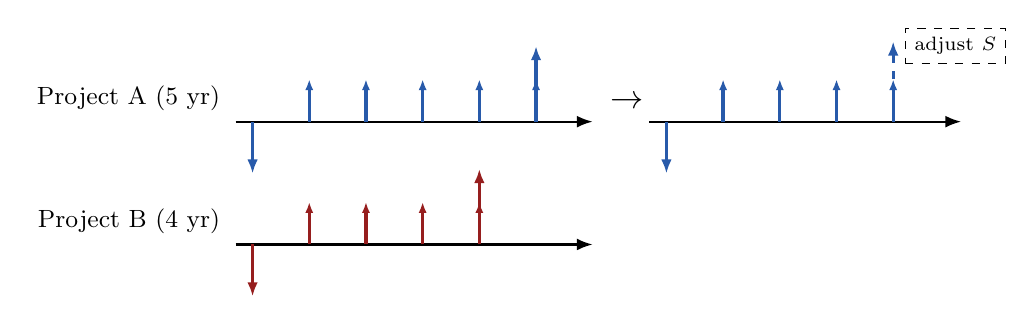
\begin{tikzpicture}[yscale=0.6,xscale=0.72]
  % Project A 5 yr, then terminated at 4 with adjusted S
  \draw[-{Latex[length=2mm]},thick] (-0.3,0) -- (6,0);
  \foreach \x in {1,...,5}{\draw[-{Latex[length=1.4mm]},very thick,negflow] (\x,0) -- (\x,0.9);}
  \draw[-{Latex[length=1.8mm]},very thick,negflow] (5,0) -- (5,1.6);
  \draw[-{Latex[length=1.8mm]},very thick,negflow] (0,0) -- (0,-1.1);
  \node[left] at (-0.4,0.5){\small Project A (5 yr)};
  \node at (6.6,0.4){\large $\rightarrow$};
  \begin{scope}[xshift=7.3cm]
  \draw[-{Latex[length=2mm]},thick] (-0.3,0) -- (5.2,0);
  \foreach \x in {1,...,4}{\draw[-{Latex[length=1.4mm]},very thick,negflow] (\x,0) -- (\x,0.9);}
  \draw[-{Latex[length=1.8mm]},very thick,negflow,dashed] (4,0.9) -- (4,1.7);
  \draw[-{Latex[length=1.8mm]},very thick,negflow] (0,0) -- (0,-1.1);
  \node[draw,dashed,anchor=west] at (4.2,1.6){\scriptsize adjust $S$};
  \end{scope}
  % Project B 4 yr
  \begin{scope}[yshift=-2.6cm]
  \draw[-{Latex[length=2mm]},thick] (-0.3,0) -- (6,0);
  \foreach \x in {1,...,4}{\draw[-{Latex[length=1.4mm]},very thick,accent] (\x,0) -- (\x,0.9);}
  \draw[-{Latex[length=1.8mm]},very thick,accent] (4,0) -- (4,1.6);
  \draw[-{Latex[length=1.8mm]},very thick,accent] (0,0) -- (0,-1.1);
  \node[left] at (-0.4,0.5){\small Project B (4 yr)};
  \end{scope}
\end{tikzpicture}
\caption*{Study period: terminate the longer project (A) at the end of the shorter one (B), replacing its salvage with an adjusted value at that time.}
\end{figure}

We already know $PW_{\text{Lexus}}(5\text{ yr}) = 4822$. Now terminate the Honda
at 5 years (instead of 10) and estimate its value at year 5 as \$7000 (the
adjusted salvage), then compute its PW:
\[
PW_{\text{Honda}}(5\text{ yr}) = -20{,}000 + 3000\,(P/A, 5\%, 5) + 7000\,(P/F, 5\%, 5) = -1527.
\]
\begin{center}
\small
\begin{tabular}{lrr}
\toprule
 & \textcolor{cHonda}{\textbf{Honda Civic}} & \textcolor{cLexus}{\textbf{Lexus RX}}\\
\midrule
FC & \textcolor{cHonda}{\$20{,}000} & \textcolor{cLexus}{\$40{,}000}\\
Annual benefit $-$ cost & \textcolor{cHonda}{\$3{,}000} & \textcolor{cLexus}{\$8{,}000}\\
Life & \textcolor{cHonda}{\textbf{5} (was 10) years} & \textcolor{cLexus}{\textbf{5 years}}\\
Salvage Value & \textcolor{cHonda}{\textbf{\$7{,}000} (was \$4{,}000)} & \textcolor{cLexus}{\$13{,}000}\\
MARR & \textcolor{cHonda}{5\%} & \textcolor{cLexus}{5\%}\\
\bottomrule
\end{tabular}
\end{center}
Since $PW_{\text{Lexus}}(5\text{ yr}) = 4822 > PW_{\text{Honda}}(5\text{ yr}) = -1527$,
the Lexus wins under the study period method too.

\begin{figure}[h]
\centering
\begin{tikzpicture}[yscale=0.68,xscale=0.78]
  \draw[-{Latex[length=2mm]},thick,cHonda] (-0.3,0) -- (6,0) node[right]{\small yr};
  \foreach \x in {1,...,5}{\draw[-{Latex[length=1.4mm]},very thick,cHonda] (\x,0) -- (\x,0.9);}
  \draw[-{Latex[length=1.8mm]},very thick,cHonda,dashed] (5,0) -- (5,1.7);
  \draw[-{Latex[length=1.8mm]},very thick,cHonda] (0,0) -- (0,-1.2);
  \node[cHonda,below] at (0,-1.2){\scriptsize 20{,}000};
  \node[cHonda,above] at (1.8,0.9){\scriptsize 3000};
  \node[cHonda,above] at (5,1.7){\scriptsize 7000 (adjusted)};
\end{tikzpicture}
\caption*{Honda terminated at year 5 with an estimated \$7000 salvage, so it can be compared with the Lexus over the same 5 years.}
\end{figure}

\begin{genform}
\[
PW = -FC + (B - C)\,(P/A, i, T) + S'\,(P/F, i, T),
\]
\where{$T=$ study period (a common horizon chosen for all alternatives, often the
shorter life);\;
$S'=$ adjusted salvage, i.e.\ the estimated value of the asset at time $T$ (not
its value at the end of its full life);\;
every other symbol is as before. Compare the $PW$ (or $AW$) of each alternative
over the same $T$ and pick the best.}
\end{genform}

\end{document}
